\documentclass{report}
% for dvips color names such as JungleGreen
% MUST come before \usepackage{tikz}
\usepackage[usenames, dvipsnames]{color}
% for \begin{lstlisting}
\usepackage{listings}
\usepackage{tikz}
\usetikzlibrary{arrows}
\usetikzlibrary{decorations.markings}
\usetikzlibrary{decorations.pathreplacing}
% For <>| See "Special Characters.rtfd"
\usepackage[T1]{fontenc}% For being able to name paths and finding their intersection. For example: "\path [name path=upward line]".
\usetikzlibrary{intersections}


\begin{document}



\begin{figure}[h]
\centering
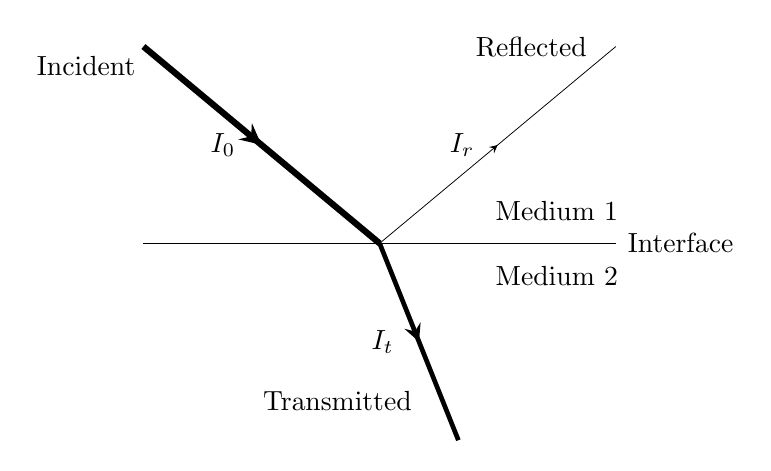
\begin{tikzpicture}
%\draw[help lines] (0,0) grid (6,5);

\draw[ultra thin](0,2.5)--(6,2.5) node[very near end,above=5pt] {Medium 1} node[very near end,below=5pt] {Medium 2} node[at end,right=1pt] {Interface};
\draw[
	line width=.8mm,
	decoration={
		markings,
		mark=at position .5 with{\arrow{stealth};}},
	postaction={decorate}](0,5)--(3,2.5) node[pos=.1, left=7pt] {Incident}node[pos=.5, left=5pt] {$I_0$};
\draw[line width=.6mm,
	decoration={
		markings,
		mark=at position .5 with{\arrow{stealth};}},
	postaction={decorate}](3,2.5)--(4,0) node[pos=.8, left=7pt] {Transmitted}node[pos=.5, left=5pt] {$I_t$};
\draw[line width=.1mm,
	decoration={
		markings,
		mark=at position .5 with{\arrow{stealth};}},
	postaction={decorate}](3,2.5)--(6,5) node[pos=1, left=7pt] {Reflected}node[pos=.5, left=5pt] {$I_r$};



\end{tikzpicture}
\label{Figure:IncidentTransmittedReflected}
\caption{The incident intensity is partly transmitted (refracted) into medium 2 and partly reflected back into medium 1}
\end{figure}



\end{document}

